% MplTplt - Yet another LaTeX template for Modern Physics Lab, PKU.
% Copyright (C) 2014 Huang Kangjing and contributors

% This work is completely rewritten basing on the work of Cao Chuanwu
% and Sun Sibai, with texts in the template originally coming from the
% Modren Phys. Lab.

% This file is released under the MIT license.
%
% Permission is hereby granted, free of charge, to any person obtaining a copy
% of this software and associated documentation files (the "Software"), to deal
% in the Software without restriction, including without limitation the rights
% to use, copy, modify, merge, publish, distribute, sublicense, and/or sell
% copies of the Software, and to permit persons to whom the Software is
% furnished to do so, subject to the following conditions:
% 
% The above copyright notice and this permission notice shall be included in
% all copies or substantial portions of the Software.
% 
% THE SOFTWARE IS PROVIDED "AS IS", WITHOUT WARRANTY OF ANY KIND, EXPRESS OR
% IMPLIED, INCLUDING BUT NOT LIMITED TO THE WARRANTIES OF MERCHANTABILITY,
% FITNESS FOR A PARTICULAR PURPOSE AND NONINFRINGEMENT. IN NO EVENT SHALL THE
% AUTHORS OR COPYRIGHT HOLDERS BE LIABLE FOR ANY CLAIM, DAMAGES OR OTHER
% LIABILITY, WHETHER IN AN ACTION OF CONTRACT, TORT OR OTHERWISE, ARISING FROM,
% OUT OF OR IN CONNECTION WITH THE SOFTWARE OR THE USE OR OTHER DEALINGS IN
% THE SOFTWARE.
%

% This template depends on the "revtex4.1" package from APS Journals
% <http://publish.aps.org/revtex/revtex-faq>, and the Chinese handling
% is done with XeLaTeX engine and package "xeCJK". Please ensure these
% packages are available in your chosen Tex software distribution.

% Document created using this template should be compiled with XeLaTeX
% engines rather than plain LaTeX or plain TeX engines.

% The non-ASCII texts of this template is encoded in UTF-8 encoding.
% Please note that XeLaTeX only accepts UTF-8 encoded documents, so
% set your editor to use UTF-8 while creating documents with this template.

% Recommended TeX software distribution to use with this template is
% Tex Live developed by the TeX User Group (TUG), please visit the home
% page of the distribution <https://www.tug.org/texlive/> for further details.

% NOTE THAT IMPORTANT INSTRUCTIONS HAS BEEN WRITTEN AS UPPERCASE COMMENTS
% IN THE TEXT, PLEASE READ THEM CAREFULLY AND FOLLOW THEM TO MAKE THE
% TEMPLATE WORK!

% Any further contributions to the template is welcome, please send
% pull requests through github or send mail to maintainer.

% For any other questions, please do not hesitate to contact maintainer.

% Current maintainer:
% Huang Kangjing <huangkangjing@gmail.com>

% Contributors:
% Sun Sibai <niasw@pku.edu.cn>
% Cao Chuanwu <>
% Huang Kangjing <huangkangjing@gmail.com>


\documentclass[aps,pre,12pt,preprint,onecolumn,showpacs,showkeys]{revtex4-1}

% Setting up Chinese handling.
\usepackage{fontspec,xeCJK}

% Setting up fonts.
% PLEASE MODIFY ALL THESE FONT NAMES ACCORDING TO YOUR FONT
% INSTALLATION AND PERFERENCE.

% Setting up main fonts and mono fonts.
\setmainfont{Liberation Serif}
\setmonofont{Liberation Mono}
% SimSun is required font for the main body of the text.
\setCJKmainfont[AutoFakeBold=5,AutoFakeSlant]{SimSun}
\setCJKmonofont[AutoFakeBold=2,AutoFakeSlant]{SimHei}

% Setting up alternative font families.
% Note that these three fonts below are required fonts in document
% title, section headings and figure captions.
\newCJKfontfamily\heiti[AutoFakeBold=2,AutoFakeSlant]{SimHei}
\newCJKfontfamily\fangsong[AutoFakeBold=5,AutoFakeSlant]{FangSong}
\newCJKfontfamily\kaiti[AutoFakeBold=5,AutoFakeSlant]{KaiTi}

% Setting up paragraph indent.
\parindent 2em

% Setting up macros for Chinese-style font size setting.
\newcommand{\fseight}{\fontsize{5.02}{6.02}\selectfont}
\newcommand{\fsseven}{\fontsize{5.52}{6.62}\selectfont}
\newcommand{\fsssix}{\fontsize{6.52}{7.83}\selectfont}
\newcommand{\fssix}{\fontsize{7.53}{9.03}\selectfont}
\newcommand{\fssfive}{\fontsize{9.03}{10.84}\selectfont}
\newcommand{\fsfive}{\fontsize{10.54}{12.65}\selectfont}
\newcommand{\fssfour}{\fontsize{12.05}{14.45}\selectfont}
\newcommand{\fsfour}{\fontsize{14.05}{16.86}\selectfont}
\newcommand{\fssthree}{\fontsize{15.06}{18.07}\selectfont}
\newcommand{\fsthree}{\fontsize{16.06}{19.27}\selectfont}
\newcommand{\fsstwo}{\fontsize{18.07}{21.68}\selectfont}
\newcommand{\fstwo}{\fontsize{22.08}{26.50}\selectfont}
\newcommand{\fssone}{\fontsize{24.09}{28.91}\selectfont}
\newcommand{\fsone}{\fontsize{26.10}{31.32}\selectfont}
\newcommand{\fsszero}{\fontsize{36.14}{43.36}\selectfont}
\newcommand{\fszero}{\fontsize{42.16}{50.59}\selectfont}

% Replace words to Chinese corespondence.
\renewcommand\appendixname{附录}
\renewcommand\abstractname{}
\renewcommand\tablename{表}
\renewcommand\figurename{图}

% Replace words in revtex4-1 to Chinese corespondence.
\makeatletter
\def\@pacs@name{\heiti\fssfour \textbf{PACS码:}\normalfont}
\def\@keys@name{\heiti\fssfour \textbf{关键词:}\normalfont}
\def\Dated@name{日期:}
\def\Received@name{\fssfive 接收 }
\def\Revised@name{\fssfive 修订 }
\def\Accepted@name{\fssfive 采纳 }
\def\Published@name{\fssfive 发表 }
\makeatother

% Change label style of enumerate.
\renewcommand{\labelenumi}{\alph{enumi}.}

% Setting up geometry.
\usepackage{geometry}
\geometry{top=2.54cm,bottom=2.54cm,left=3cm,right=3cm}

% Setting up line space.
\usepackage{setspace}
\linespread{1.6}

% Setting up hyperreferences.
\usepackage{hyperref}
\hypersetup{colorlinks=true}

% Setting up styles for section headings.
\usepackage{titlesec}
\titleformat*{\section}{\bf\fangsong\fsfour}
\titleformat*{\subsection}{\bf\fangsong}

% Loading packages for image handling.
\usepackage{subfig}
\usepackage{graphicx,psfrag,epsfig}

% Setting up caption styles.
\usepackage{caption}
\DeclareCaptionFont{kaiti}{\kaiti}
\DeclareCaptionFont{bfheiti}{\bf\heiti}
\captionsetup{font=small,format=plain,labelfont=bfheiti,%
  textfont=kaiti,justification=raggedright,%
  singlelinecheck=false}

% Loading packages for math typings.
\usepackage{amsmath,amsfonts,amssymb,amsthm,bm,upgreek}
\usepackage[mathscr]{eucal}
\usepackage{siunitx}
\usepackage{listings,color}
\lstset{%
    breaklines=true,
    basicstyle=\fontspec{Liberation Mono}\footnotesize,
    commentstyle=\fontspec{Liberation Mono}\it\color{green},
    showspaces=false,
    stringstyle=\fontspec{Liberation Mono}\bf,
    numbers=left,
    numberstyle=\fontspec{Liberation Mono}\tiny,
    keywordstyle=\fontspec{Liberation Mono}\bf\color{blue},
    title=\lstname,
    frame=L}


\begin{document}

% Title and author info.
\title{\bf\heiti\fsthree 用电容-电压法测量半导体中的杂质分布\vspace{15mm}}
\author{\fangsong\fsfour 黄康靖\vspace{2mm}}
\affiliation{\normalfont\fssfour 2012级~~~~学号:{masked student id}\vspace{2mm}}
\date{\today}
\keywords{半导体,杂质分布,锁定放大器,电容,电压}
\email{huangkangjing@gmail.com}

% Abstract.
\begin{abstract}
  \vspace{10mm}
  \begin{spacing}{1.5}
    \fssfour
    在现代半导体物理学中,掺杂半导体中的杂质分布是半导体材料的一个重要属性.半导体
    工艺的相关设计和原理都依赖于这个属性.本实验利用锁定放大器放大小电压信号,使用
    电容-电压法原理,测得了p$^+$-n结中n型半导体一侧的半导体材料杂质分布曲线.
  \end{spacing}
\end{abstract}

% The main body of the document goes from here.
\maketitle
\fssfour
\section{引言}

半导体物理学中,半导体器件设计与制造的核心问题是如何控制半导体内的杂质分布,以满足
半导体器件实际应用的需要.基于这个原因,正确地检测杂志浓度及其分布是制备合格半导体
器件的必要条件.所以杂质的浓度及其分布的测量是半导体材料及器件研究中的基本测量之
一.通过测量不同直流偏压下p-n结势垒电容,可以在不破坏器件本身的情况下比较迅速地测
得单边突变p-n结中,轻掺杂一侧的半导体的杂质浓度及其分布.

本实验利用上述的这一C-V法,使用锁定放大器与函数信号记录仪等仪器,测量了p$^+$-n结轻
掺杂一侧的杂质浓度及其分布.

\section{原理}

\subsection{p-n结的势垒电容与杂质浓度的关系}

我们知道,当n型半导体与p型半导体在某一界面上相互接触时,由于两种半导体中的载流子种
类与符号不同,p型半导体中的空穴将会扩散到空穴较少的n型半导体去,而n型半导体中的电
子将会扩散到空穴较少的p型半导体中去.然而,在交接面上,两种载流子会相互湮灭,从而产
生没有载流子,有空间净电荷分布的耗尽区.耗尽区内的电场使得载流子在其中作漂移运动.
这两种因素相互竞争的结果即是耗尽区的宽度达到了一个动态平衡,即为p-n结的宽度.

当空间电荷区域宽度变化$dw$时,相应的单位面积的空间电荷变化量
\begin{equation}
    dQ = qN(w)dw
\end{equation}
其中$N(w)$是空间电荷区域宽度$w$边界处的杂质浓度,增加的电荷$dQ$将引起电场改变
$dE$,由泊松方程可以求得
\begin{equation}
    dE = \frac{dQ}{\epsilon\epsilon_0}
\end{equation}
相应地
\begin{equation}
    d(V_R + V_D) = dV_R = wdE
\end{equation}
以上两式消去$dE$,得
\begin{equation}
    \label{C-w}
    \frac{dQ}{dV_R} = \frac{\epsilon\epsilon_0}{w} = \frac{C}{A}
\end{equation}
整理得到
\begin{equation}
    \label{formula}
    \begin{split}
    N(w) = & \frac{2}{q\epsilon\epsilon_0A^2}\frac{1}{\frac{d(1/C^2)}{dV_R}} \\
    = & -\frac{1}{q\epsilon\epsilon_0A^2}\frac{C^3}{dC/dV_R}
    \end{split}
\end{equation}

对于p$^+$-n结来说,我们有关系$N_A \gg N_D$,那么$x_n \gg x_p$, 于是总空间电荷区宽
度$w = x_n + x_p \approx x_n$,那么,我们得到的$N(w)$分布近似上就是n侧半导体内杂质
浓度随深度的变化分布.

从此式我们可以看到,只要求得C-V曲线,按式~\ref{formula}再结合式~\ref{C-w}即可算出
杂质的分布情况.

\subsection{势垒电容的测量}

p-n结势垒电容是一个随直流偏压变化的微分电容,测量时采取的方法是在p-n结上偏置一定
的反向直流偏压$V_R$,同时再在$V_R$上叠加一个微小的交变电压信号$v(t)$,这信号经过待
测的p-n结电容$C_x$和一个与之相串接的已知电容$C_0$,当$C_0 \gg C_X$时,在$C_0$两端
的电压为:
\begin{equation}
   v_i = \frac{v(t)}{\frac{1}{j\omega C_x} + \frac{1}{j\omega
           C_0}}\cdot\frac{1}{j\omega C_0} \approx \frac{C_x}{C_0} v(t)
\end{equation}
通过这一线性关系,即可测得$C_x$的值.

\section{实验}

实验的测量方框图如图~\ref{fig:ins}所示.图中的单刀双掷开关是为了切换测量实际容值
和校准锁定放大器的测量信号输出而设计的.$D_1$,$D_2$两个二极管和旁的电容组成的电路
是锁定放大器的输入保护电路.

\begin{figure}[htbp]
    \centering
    \includegraphics[width=\textwidth]{drawing.pdf}
    \caption{\label{fig:ins}
        实验装置的测量方框图,图中锁定放大器型号为Model 128 Lock-in Amplifier}
\end{figure}

在本实验中,锁定放大器主要起到从噪声中提取固定频率的信号,并且将其放大到可以测量的
幅度的作用.

我们知道,在半导体电子学实验中,由于实验器材和实验素材的不可避免的缺陷和涨落因素,
在电路中会存在各种噪音,影响实验的测量.本次实验中,由于实验的测量信号$v_i$十分微弱
,这一问题显得尤为显著.而锁定放大器是一种交流电压表,它通过相敏检波器和低通滤波器
,实现了测量深埋在噪声之中的周期重复信号的幅值与相位的能力,本实验正是利用它的这一
能力,进行实验数据的测量.

本实验分以下三个部分进行:

\begin{enumerate}
    \item 通过若干个标准电容的测量,证实了锁定放大器的输出与被测电容之间的线性关
        系
    \item 实验的二极管样品有若干由于在反向加电压时会被击穿,从而不适合测量.击穿现
        象表现为在反向加电压时由于反向漏电电流较大且随加的反向电压变化,从而导致
        其相位会发生变化.实验甄别了可用于测量的二极管.
    \item 实验测量了选定二极管样品的C-V特性曲线,从而在此基础上计算出了杂质分布曲
        线.
\end{enumerate}

\section{实验结果及分析讨论}

\subsection{锁定放大器输出电压与被测电容之间的线性关系}

\begin{figure}
\begin{center}
    \includegraphics[width=\textwidth]{plot1.pdf}
\end{center}
\caption{\label{fig:plot1}本图是锁定放大器输出电压与被测电容之间的线性关系的验证
性测量的测量图线.图中蓝色线条为线性拟合线条,黑色标记为测量数据点.图上所写$r$值为
拟合所得的线性相关系数}
\end{figure}


这一线性关系的证实性测量结果如图~\ref{fig:plot1}所示.

从图表中可以看出,证实性测量基本证实了这两个物理量之间的线性关系,并且这一线性关系
吻合的非常好,这意味着我们的测量系统是满足条件$C_0 \gg C_x$的

\subsection{可用二极管的确定}

经过相位-反向电压关系的测量,我们确定了一号和二号二极管的端电压相位是不基本不随电
压值变化的,可用于本实验测量.


\subsection{杂质分布的测定}

我们选定二号二极管进行杂质分布的测量,首先,我们测得二号二极管上的电容电压关系如图~\ref{uc}所示.

\begin{figure}
\begin{center}
    \includegraphics[width=\textwidth]{uc.pdf}
\end{center}
\caption{\label{uc}二号二极管上的电容电压关系测量曲线,由函数记录仪记录下来并且扫
描进计算机后经过程序处理提取数据得到}
\end{figure}

基于测得的电容电压关系图线,可以得到电容对电压的导数随电压的变化曲线如图~\ref{diff}所示.

\begin{figure}
\begin{center}
    \includegraphics[width=\textwidth]{diff.pdf}
\end{center}
\caption{\label{diff}二号二极管上的电容对电压导数与电压的关系图线,由电容电压关系
图线计算得到}
\end{figure}

最后,基于式~\ref{formula}我们可以得到待测样品中杂质的分布图线如图~\ref{Nw}所示.


\begin{figure}
\begin{center}
    \includegraphics[width=\textwidth]{Nw.pdf}
\end{center}
\caption{\label{Nw}最终测得的样品中杂质分布曲线,注意其中有些点没有数值,这是因为
数值微分的误差,导致这些点的电容对电压导数为0,从而按式~\ref{formula}这里的分布值
没有定义}
\end{figure}



\section{结论}

本实验通过电容电压法,利用锁定放大器测量微小电压,在此基础上成功地测得了p$^+$-n结
中n型半导体侧的杂质浓度分布.

\section{致谢}

感谢在实验中许福军老师细致而专业的指导


\begin{thebibliography}{}
\bibitem{book} 吴思成,王祖铨~2010 近代物理实验(第三版)(北京:高等教
育出版社)第412页.  %实验书
\end{thebibliography}

\clearpage
\appendix

\section{代码}

本实验的所有数据处理和绘图使用python语言完成.具体的处理使用了python的numpy,scipy
和matplotlib这数个开放源代码库套件.

相关的处理代码附在文后

\lstinputlisting[language=python]{data.py}
\lstinputlisting[language=python]{diff.py}
\lstinputlisting[language=python]{linear.py}
\lstinputlisting[language=python]{N.py}
\lstinputlisting[language=python]{uc.py}

\end{document}
